Il seguente listato genera due grafici per le funzioni date:
\lstinputlisting[language=Matlab]{cap_4/es2/es2.m}
\lstinputlisting[language=Matlab]{cap_4/es2/evaluate_poli.m}
\lstinputlisting[language=Matlab]{cap_4/ascisseEquispaziate.m}
\lstinputlisting[language=Matlab]{cap_4/chebyshev.m}

\global\csname @topnum\endcsname 0
\begin{figure}
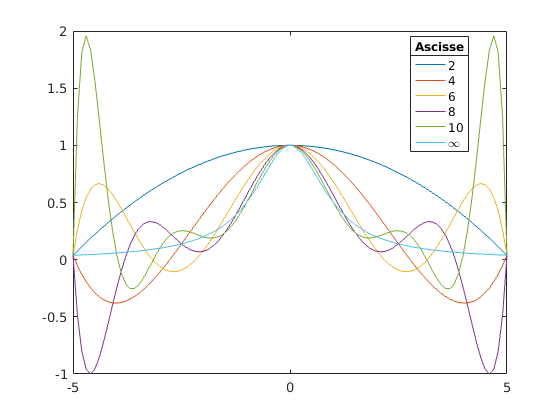
\includegraphics[width=\textwidth]{cap_4/es2/Runge_equi.png}
\caption{Ascisse Equidistanti per $f(x) = \frac{1}{1+x^2}$}
\label{RungeEq}
\end{figure}
\begin{figure}
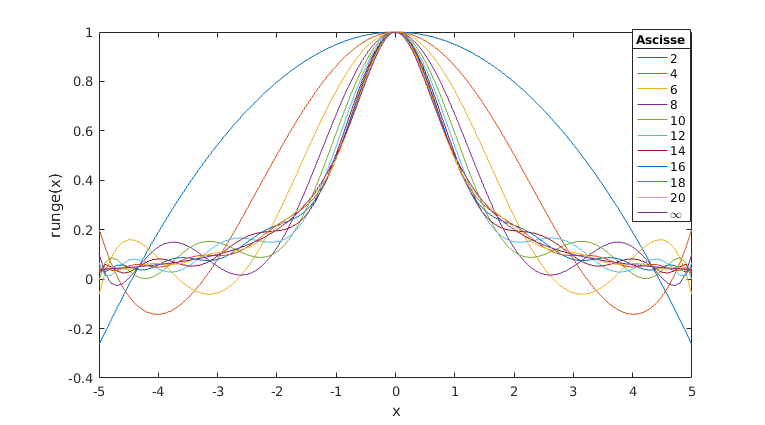
\includegraphics[width=\textwidth]{cap_4/es2/Runge_cheb.png}
\caption{Ascisse di Chebyshev per $f(x) = \frac{1}{1+x^2}$}
\label{RungeChe}
\end{figure}
\begin{figure}
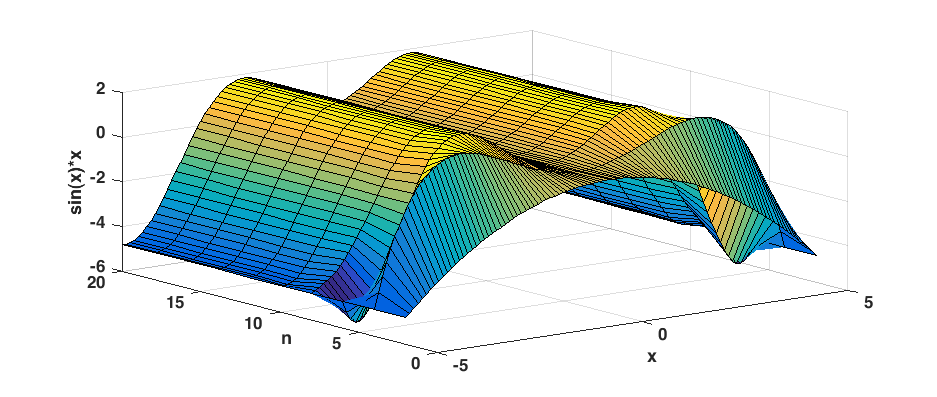
\includegraphics[width=\textwidth]{cap_4/es2/Sin_equi.png}
\caption{Ascisse Equidistanti per $g(x) = sin(x)*x$}
\label{SinEq}
\end{figure}
\begin{figure}
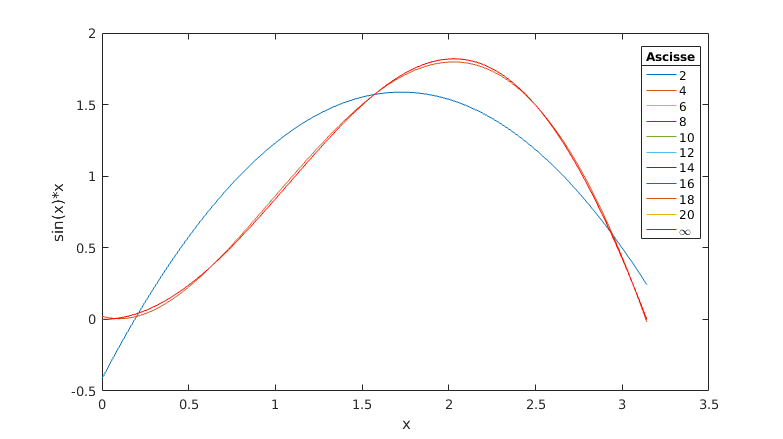
\includegraphics[width=\textwidth]{cap_4/es2/Sin_cheb.png}
\caption{Ascisse di Chebyshev per $g(x) = sin(x)*x$}
\label{SinChe}
\end{figure}

\begin{figure}
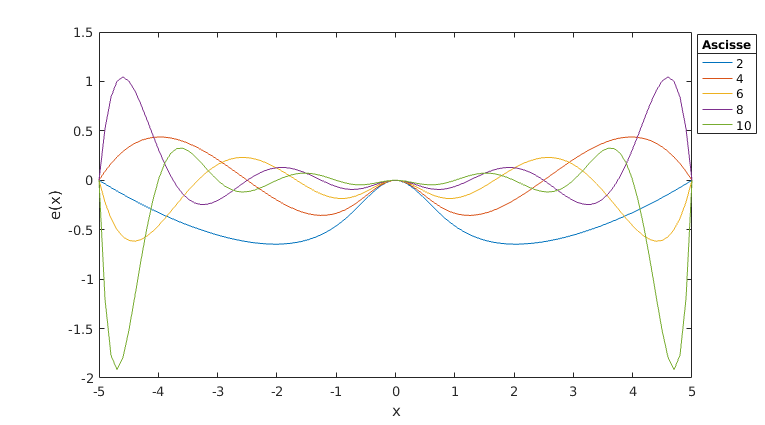
\includegraphics[width=\textwidth]{cap_4/es2/Runge_equi_err.png}
\caption{Errore per Ascisse Equidistanti per $f(x) = \frac{1}{1+x^2}$}
\label{RungeEqErr}
\end{figure}
\begin{figure}
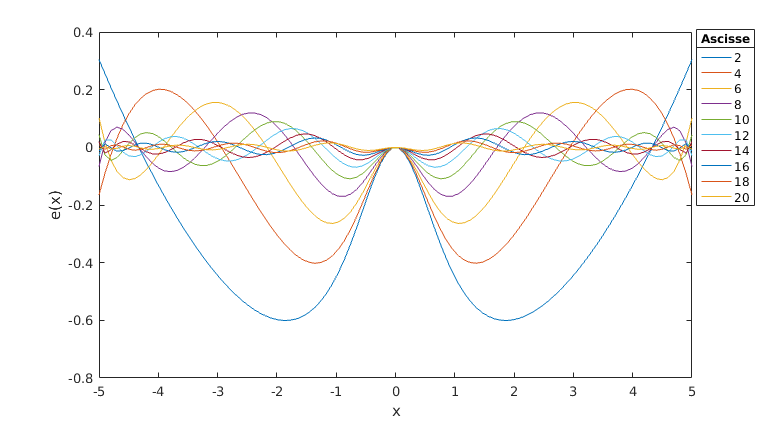
\includegraphics[width=\textwidth]{cap_4/es2/Runge_cheb_err.png}
\caption{Errore per Ascisse di Chebyshev per $f(x) = \frac{1}{1+x^2}$}
\label{RungeCheErr}
\end{figure}
\begin{figure}
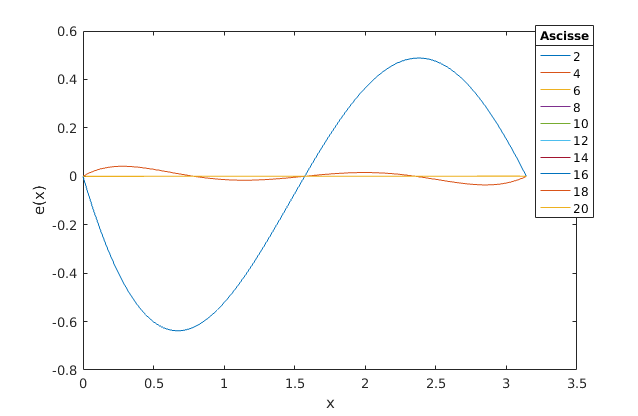
\includegraphics[width=\textwidth]{cap_4/es2/Sin_equi_err.png}
\caption{Errore per Ascisse Equidistanti per $g(x) = sin(x)*x$}
\label{SinEqErr}
\end{figure}
\begin{figure}
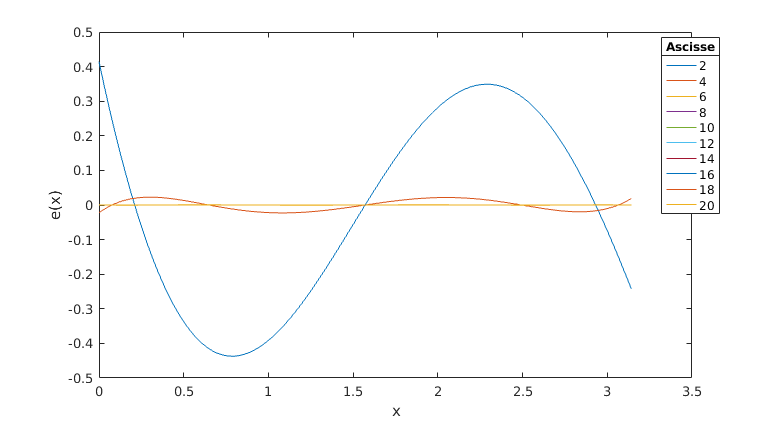
\includegraphics[width=\textwidth]{cap_4/es2/Sin_cheb_Err.png}
\caption{Errore per Ascisse di Chebyshev per $g(x) = sin(x)*x$}
\label{SinCheErr}
\end{figure}
$\left(\begin{tabu}{cccc}
RungeEq & RungeCheb & SinEq & SinCheb \\
\hline
0.646 & 0.4371 & 0.6381 & 0.4371\\ 0.4383 & 0.02286 & 0.04127 & 0.02286\\ 0.6164 & 0.0004779 & 0.001343 & 0.0004779\\ 1.045 & 5.332\cdot 10^{-6} & 2.575\cdot 10^{-5} & 5.332\cdot 10^{-6}\\ 1.915 & 3.688\cdot 10^{-8} & 3.238\cdot 10^{-7} & 3.688\cdot 10^{-8}\\ 3.612 & 1.734\cdot 10^{-10} & 2.843\cdot 10^{-9} & 1.734\cdot 10^{-10}\\ 7.189 & 5.892\cdot 10^{-13} & 1.873\cdot 10^{-11} & 5.892\cdot 10^{-13}\\ 14.01 & 3.417\cdot 10^{-15} & 1.261\cdot 10^{-13} & 3.417\cdot 10^{-15}\\ 27.51 & 1.776\cdot 10^{-15} & 8.933\cdot 10^{-14} & 1.776\cdot 10^{-15}\\ 58.41 & 2.327\cdot 10^{-15} & 1.768\cdot 10^{-13} & 2.327\cdot 10^{-15} \end{tabu}\right)$


Possiamo vedere la differenza tra \ref{RungeEq} e \ref{RungeChe}, nella prima all'aumentare delle ascisse la funzione interpolata degenera, mentre nella seconda già con n=5 abbiamo una buona interpolazione.
Nel caso della seconda funzione possiamo vedere che la differenza tra \ref{SinEq} e \ref{SinChe} non è molto rilevante. Infatti già con 4 ascisse abbiamo un interpolazione quasi perfetta.
Nelle figure \ref{RungeEqErr} \ref{RungeCheErr} \ref{SinEqErr} \ref{SinCheErr} e' possibile vedere l'andamento dell'errore per i vari metodi di interpolazione.
